% ===========================================================================
%  PART IV --- PROXIMAL POLICY OPTIMIZATION (Schulman et al., 2017)
% ===========================================================================
\clearpage
\part{Proximal Policy Optimization}

\partintro{\textbf{The question of Part IV:} TRPO's second-order step uses each batch \textbf{once}. PPO wants \textbf{many first-order SGD steps} per batch without leaving the trust region. It \textbf{clips} the importance ratio, so the objective itself stops rewarding large moves.}

% ---------------------------------------------------------------------------
\section{Setting and motivation}
% ---------------------------------------------------------------------------

\paper{Proximal Policy Optimization Algorithms}
  {Schulman, Wolski, Dhariwal, Radford \& Klimov}{arXiv 2017 (OpenAI)}
  {PPO --- TRPO's reliability with only first-order SGD}
  {proximal\_policy\_optimization\_algorithms.md}

\begin{itemize}
  \item Same setting as TRPO; advantages $\hat A_t$ from (truncated) \textbf{GAE}.
  \item \textbf{TRPO}: complicated; no dropout, no parameter sharing between policy and value.
  \item \textbf{Vanilla PG}: several steps on the same batch $\Rightarrow$ destructively large updates.
  \item \textbf{Goal}: reuse each batch for many SGD steps, without leaving the trust region.
  \item Tested on MuJoCo and 49 Atari games.
\end{itemize}

\begin{notebox}
``Vanilla'' PG estimator: $\hat g=\hat\E_t[\nabla_\theta\log\pi_\theta(a_t\mid s_t)\hat A_t]$, from the loss $L^{PG}=\hat\E_t[\log\pi_\theta\,\hat A_t]$; $\hat\E_t$ is the empirical average over a batch. Q-learning with function approximation is also dismissed: it fails on many simple problems and had no strong continuous-control results at the time.
\end{notebox}

\subsection{The goal: many SGD steps per batch}

\begin{center}
\begin{tikzpicture}[x=0.62cm, y=1cm, font=\scriptsize]
  \node[font=\small\bfseries, anchor=east] at (-0.2,1.3) {TRPO};
  \foreach \a/\b in {0/3, 3.6/6.6, 7.2/10.2, 10.8/13.8} {
    \fill[AtlasSlate!25] (\a,1.1) rectangle (\b,1.5); \node at ({(\a+\b)/2},1.3) {collect};
    \fill[AtlasWarm] (\b,1.1) rectangle (\b+0.6,1.5);}
  \node[font=\small\bfseries, anchor=east, text=AtlasCool] at (-0.2,0.3) {PPO};
  \foreach \a/\b in {0/3, 5.4/8.4, 10.8/13.8} {
    \fill[AtlasSlate!25] (\a,0.1) rectangle (\b,0.5); \node at ({(\a+\b)/2},0.3) {collect};}
  \foreach \b in {3, 8.4} {
    \foreach \k in {0,...,5} \fill[AtlasCool] (\b+\k*0.4,0.1) rectangle (\b+\k*0.4+0.3,0.5);}
  \draw[decorate, decoration={brace, amplitude=3pt, mirror}] (3,0.0) -- node[below=3pt, text=AtlasCool]{$K$ epochs, minibatches} (5.4,0.0);
  \fill[AtlasWarm] (0,2.0) rectangle (0.4,2.3); \node[anchor=west] at (0.45,2.15) {one policy update};
  \fill[AtlasSlate!25] (5,2.0) rectangle (5.4,2.3); \node[anchor=west] at (5.45,2.15) {environment samples};
\end{tikzpicture}
\end{center}

\begin{pair}
\begin{slatebox}[title={TRPO}]
\small One (expensive, carefully constrained) step, then the batch is thrown away.
\end{slatebox}
\begin{coolbox}[title={PPO}]
\small Squeeze the same batch with cheap first-order steps: $K$ epochs of minibatch SGD.
\end{coolbox}
\end{pair}

\begin{warnbox}[title={Why naive reuse fails}]
The data came from $\piold$: the surrogate is trustworthy only near $r_t=1$. For one sample with $\hat A_t>0$ the term $r_t\hat A_t$ is linear in $r_t$ --- \textbf{nothing says stop}. Unchecked, repeated steps give \textbf{destructively large} updates. Only TRPO's KL constraint stopped it; PPO asks how to stop it with an ordinary first-order optimizer.
\end{warnbox}

% ---------------------------------------------------------------------------
\section{Back to the CPI surrogate}
% ---------------------------------------------------------------------------

The ratio is TRPO's importance weight:
\begin{gather*}
  r_t(\theta) = \frac{\pi_\theta(a_t\mid s_t)}{\pi_{\told}(a_t\mid s_t)}, \qquad r_t(\told)=1.
\end{gather*}

\begin{eqbox}
\begin{gather*}
  L^{CPI}(\theta) = \hat\E_t\big[r_t(\theta)\,\hat A_t\big] \qquad \text{(``CPI'': Kakade \& Langford, where this objective was proposed)}
\end{gather*}
\end{eqbox}

{\small It is TRPO's $L_{\told}$ written with sample averages; its gradient at $\told$ is the vanilla policy gradient. Many SGD steps on $L^{CPI}$ alone: $r_t$ runs far from 1 $\Rightarrow$ huge updates. Normalized score $-0.39$: worse than random (\S\ref{sec:ppo-ablation}).}

\textbf{Three ways to stay close:}

\begin{pair}[3]
\begin{slatebox}[title={Constraint (TRPO)}]
\small s.t.\ $\hat\E_t[\DKL]\le\delta$\\[2pt]
{\scriptsize second-order solver}
\end{slatebox}
\begin{warmbox}[title={Penalty (baseline)}]
\small $-\beta\,\hat\E_t[\DKL]$\\[2pt]
{\scriptsize no single $\beta$ works $\to$ adapt it}
\end{warmbox}
\begin{coolbox}[title={Clip (``PPO'')}]
\small no gain once $|r_t-1|>\epsilon$\\[2pt]
{\scriptsize first order}
\end{coolbox}
\end{pair}

{\small The penalty form is what TRPO's theory suggests; TRPO used a constraint because ``it is hard to choose a single value of $\beta$ that performs well across different problems --- or even within a single problem''.}

% ---------------------------------------------------------------------------
\section{The clipped surrogate objective}
% ---------------------------------------------------------------------------

\begin{eqbox}
\begin{gather*}
  L^{CLIP}(\theta) = \hat\E_t\Big[\min\big(r_t(\theta)\hat A_t,\ \mathrm{clip}(r_t(\theta),1-\epsilon,1+\epsilon)\,\hat A_t\big)\Big],
  \qquad \epsilon = 0.2
\end{gather*}
\end{eqbox}

One term of the sum, as a function of the ratio $r$:

\begin{center}
\begin{tikzpicture}
\begin{axis}[notes, name=pos, width=6.8cm, height=4.6cm, xmin=0, xmax=2, ymin=0, ymax=2,
    xlabel={$r$}, xtick={0.8,1,1.2}, xticklabels={$1{-}\epsilon$,1,$1{+}\epsilon$}, ytick=\empty,
    title={\small $\hat A_t>0$}, axis lines=middle, x label style={at={(axis description cs:1,0)}, anchor=west}]
  \addplot[gray, thick, dashed, domain=0:2] {x};
  \addplot[AtlasCool, very thick, domain=0:1.2] {x};
  \addplot[AtlasCool, very thick, domain=1.2:2] {1.2};
  \fill[BadRed] (axis cs:1,1) circle (2pt);
  \node[font=\scriptsize, gray] at (axis cs:1.7,1.85) {$L^{CPI}$};
  \node[font=\scriptsize, AtlasCool] at (axis cs:1.6,1.05) {$L^{CLIP}$};
\end{axis}
\begin{axis}[notes, at={(pos.east)}, anchor=west, xshift=1.2cm, width=6.8cm, height=4.6cm, xmin=0, xmax=2, ymin=-2, ymax=0,
    xlabel={$r$}, xtick={0.8,1,1.2}, xticklabels={$1{-}\epsilon$,1,$1{+}\epsilon$}, ytick=\empty,
    title={\small $\hat A_t<0$}, axis lines=middle, x label style={at={(axis description cs:1,1)}, anchor=west},
    xticklabel style={yshift=6pt}]
  \addplot[gray, thick, dashed, domain=0:2] {-x};
  \addplot[AtlasCool, very thick, domain=0:0.8] {-0.8};
  \addplot[AtlasCool, very thick, domain=0.8:2] {-x};
  \fill[BadRed] (axis cs:1,-1) circle (2pt);
  \node[font=\scriptsize, AtlasCool] at (axis cs:0.35,-0.65) {$L^{CLIP}$};
\end{axis}
\end{tikzpicture}\\
{\scriptsize Redrawn from PPO Fig.~1. Red dot: the start of the optimization, $r=1$. Dashed: $L^{CPI}$.}
\end{center}

\begin{pair}
\begin{coolbox}[title={$\hat A_t>0$: raise $\pi(a_t\mid s_t)$}]
\small
\begin{itemize}
  \item No extra gain past $1+\epsilon$ (flat).
  \item Wrong way ($r<1-\epsilon$): \textbf{not} clipped, still costs.
\end{itemize}
\end{coolbox}
\begin{coolbox}[title={$\hat A_t<0$: lower $\pi(a_t\mid s_t)$}]
\small
\begin{itemize}
  \item No extra gain below $1-\epsilon$ (flat).
  \item Wrong way ($r>1+\epsilon$): \textbf{not} clipped, the loss keeps growing.
\end{itemize}
\end{coolbox}
\end{pair}

\begin{keybox}[title={A pessimistic bound}]
\begin{enumerate}
  \item The $\min$ gives $L^{CLIP}\le L^{CPI}$: clipping removes \textbf{gains}, never hides \textbf{losses}.
  \item Moving the wrong way keeps its gradient: the update can always pull $r_t$ \textbf{back} toward 1.
  \item $L^{CLIP}=L^{CPI}$ to first order at $\told$.
\end{enumerate}
\end{keybox}

{\small PPO Fig.~2: along the update direction, $L^{CLIP}$ peaks at a KL of about 0.02 (Hopper).}

\subsection{What clipping replaces}

\begin{center}
\begin{tikzpicture}[font=\footnotesize, >=Stealth,
    cr/.style={fl, line width=0.8pt, text width=3.6cm, minimum height=1.9cm, font=\footnotesize}]
  \node[cr, cbox=AtlasWarm] (c) at (0,0) {\textbf{\color{AtlasWarm}CPI}\\[2pt] mixture step\\ $\pinew=(1-\alpha)\pi+\alpha\pi'$\\[2pt] {\scriptsize close \textbf{by construction}}};
  \node[cr, cbox=AtlasSlate] (t) at (4.7,0) {\textbf{TRPO}\\[2pt] KL constraint\\ $\bar D_{\mathrm{KL}}(\told,\theta)\le\delta$\\[2pt] {\scriptsize close \textbf{by a solver} (2nd order)}};
  \node[cr, cbox=AtlasCool] (p) at (9.4,0) {\textbf{\color{AtlasCool}PPO}\\[2pt] clipped ratio\\ $r_t\in[1-\epsilon,1+\epsilon]$\\[2pt] {\scriptsize close \textbf{by the objective} (1st order)}};
  \draw[->, thick, AtlasSlate] (c) -- (t);
  \draw[->, thick, AtlasSlate] (t) -- (p);
\end{tikzpicture}
\end{center}

\textbf{Proximal} $=$ keep $\pi_\theta$ near $\piold$ --- with plain minibatch SGD/Adam, several epochs per batch.

\begin{warnbox}[title={Clipping is an incentive, not a limit}]
Clipping removes the \textbf{incentive} to move a ratio further --- it does not \textbf{enforce} a limit. Clipped samples can still drift through shared parameters, moved by the gradients of unclipped samples, so \textbf{no KL bound is guaranteed}. In practice the KL stays small; some implementations add early stopping on the KL (cf.\ Engstrom et al., 2020, ``Implementation Matters in Deep Policy Gradients'').
\end{warnbox}

% ---------------------------------------------------------------------------
\section{PPO in practice}
% ---------------------------------------------------------------------------

\begin{eqbox}
\begin{gather*}
  L_t^{CLIP+VF+S}(\theta) = \hat\E_t\Big[\underbrace{L_t^{CLIP}(\theta)}_{\text{policy}}
    - c_1\underbrace{\big(V_\theta(s_t)-V_t^{\mathrm{targ}}\big)^2}_{\text{\color{AtlasWarm}value}}
    + c_2\underbrace{S[\pi_\theta](s_t)}_{\text{entropy}}\Big]
\end{gather*}
\end{eqbox}

\begin{enumerate}
  \item $c_1$ matters only when policy and value \textbf{share parameters} (one network, one loss).
  \item The entropy bonus $S$ is PPO's only explicit exploration term (``to ensure sufficient exploration'') --- it acts on the \textbf{action} distribution, not on where episodes start.
\end{enumerate}

\begin{minipage}[t]{0.56\linewidth}
\begin{algbox}{PPO, actor--critic style (Alg.~1)}
\begin{enumerate}
  \item $N$ actors run $\pi_{\told}$ for $T$ steps each.
  \item Truncated GAE: $\hat A_t = \sum_{l=0}^{T-t-1}(\gamma\lambda)^l\delta_{t+l}$.
  \item $K$ epochs of minibatch Adam on $L$.
  \item $\told\leftarrow\theta$.
\end{enumerate}
\end{algbox}
\end{minipage}\hfill
\begin{minipage}[t]{0.4\linewidth}
\small
\begin{tabular}{l r r}
\toprule
 & \textbf{MuJoCo} & \textbf{Atari} \\
\midrule
horizon $T$ & 2048 & 128 \\
epochs $K$ & 10 & 3 \\
minibatch & 64 & $32\times8$ \\
actors $N$ & --- & 8 \\
Adam step & $3\cdot10^{-4}$ & $2.5\cdot10^{-4}\alpha$ \\
$\gamma$, $\lambda$ & 0.99, 0.95 & 0.99, 0.95 \\
clip $\epsilon$ & 0.2 & $0.1\alpha$ \\
\bottomrule
\end{tabular}\\[2pt]
{\scriptsize\color{NoteGray}PPO Tables 3, 5. Atari: $\alpha$ annealed $1\to0$, $c_1=1$, $c_2=0.01$.}
\end{minipage}

{\small $K$ epochs on the same batch is the point: TRPO took \textbf{one} step per batch. Truncated GAE does not look beyond the segment end $T$, which suits fixed-length segments and recurrent nets.}

% ---------------------------------------------------------------------------
\section{TRPO vs.\ PPO}
% ---------------------------------------------------------------------------

\begin{center}
\small
\begin{tabular}{l l l}
\toprule
 & \textbf{TRPO} & \textbf{\color{AtlasCool}PPO} \\
\midrule
stay close by & KL constraint $\bar D_{\mathrm{KL}}\le\delta$ & clipped ratio $[1-\epsilon,1+\epsilon]$ \\
solver & CG + line search (2nd order) & minibatch Adam (1st order) \\
steps per batch & one & $K$ epochs \\
policy + value & separate networks & may share (one loss) \\
advantages & Monte Carlo $\hat Q$ & truncated GAE \\
states from & $s_0\sim\rho_0$, then $\piold$ & same --- still no $\mu$ \\
\bottomrule
\end{tabular}
\end{center}

\begin{pair}
\begin{keybox}[title={Kept from CPI and TRPO}]
\begin{itemize}
  \item Surrogate on the \textbf{old} samples
  \item The ratio $\pi_\theta/\pi_{\told}$
  \item Small, controlled steps
\end{itemize}
\end{keybox}
\begin{warnbox}[title={Given up}]
\begin{itemize}
  \item Any improvement \textbf{bound}
  \item An exact limit on the KL
  \item (Monotone improvement: never had it in practice)
\end{itemize}
\end{warnbox}
\end{pair}

{\small TRPO's practical algorithm already dropped the guarantee (mean KL, fixed $\delta$, estimated advantages); PPO drops the remaining machinery and keeps the heuristic.}

% ---------------------------------------------------------------------------
\section{Results}
% ---------------------------------------------------------------------------

\subsection{Clipping vs.\ KL penalty: the ablation}
\label{sec:ppo-ablation}

\begin{minipage}[c]{0.55\linewidth}
\centering
\begin{tikzpicture}[x=3.4cm, y=0.42cm, font=\scriptsize]
  \foreach \y/\lab/\v/\c in {
      0/No clipping or penalty/-0.39/BadRed!70,
      1.3/Clipping $\epsilon=0.1$/0.76/AtlasCool!55,
      2.3/Clipping $\epsilon=0.2$/0.82/AtlasCool,
      3.3/Clipping $\epsilon=0.3$/0.70/AtlasCool!55,
      4.6/Adaptive KL $d_{\mathrm{targ}}=0.003$/0.68/AtlasWarm!55,
      5.6/Adaptive KL $d_{\mathrm{targ}}=0.01$/0.74/AtlasWarm!55,
      6.6/Adaptive KL $d_{\mathrm{targ}}=0.03$/0.71/AtlasWarm!55,
      7.9/Fixed KL $\beta=0.3$/0.62/AtlasSlate!40,
      8.9/Fixed KL $\beta=1$/0.71/AtlasSlate!40,
      9.9/Fixed KL $\beta=3$/0.72/AtlasSlate!40,
      10.9/Fixed KL $\beta=10$/0.69/AtlasSlate!40} {
    \fill[\c] (0,-\y-0.35) rectangle (\v,-\y+0.35);
    \node[anchor=east] at (-0.42,-\y) {\lab};
    \node[anchor=west, font=\tiny] at ({max(\v,0)+0.01},-\y) {$\v$};}
  \draw[gray] (0,0.8) -- (0,-11.6);
  \draw[gray, dashed] (1,0.8) -- (1,-11.6);
  \node[font=\tiny, NoteGray] at (0,-12.2) {0 = random};
  \node[font=\tiny, NoteGray] at (1,-12.2) {1 = best};
\end{tikzpicture}\\
{\scriptsize PPO Table 1: 7 MuJoCo tasks $\times$ 3 seeds, 1M steps.}
\end{minipage}\hfill
\begin{minipage}[c]{0.42\linewidth}
\begin{warmbox}[title={Adaptive KL penalty}]
\begin{gather*}
  L^{KLPEN} = \hat\E_t\big[r_t\hat A_t - \beta\,\DKL[\pi_{\told},\pi_\theta]\big]
\end{gather*}
After each update, with $d=\hat\E_t[\DKL]$:
\begin{itemize}
  \item $d < d_{\mathrm{targ}}/1.5$: \ $\beta\leftarrow\beta/2$
  \item $d > 1.5\,d_{\mathrm{targ}}$: \ $\beta\leftarrow 2\beta$
\end{itemize}
{\scriptsize Constants 1.5 and 2 are heuristic; not sensitive to them.}
\end{warmbox}
\begin{keybox}
Clipping with $\epsilon=0.2$ wins; the KL penalty stays a useful baseline.
\end{keybox}
\end{minipage}

\subsection{PPO vs.\ other algorithms}

\begin{center}
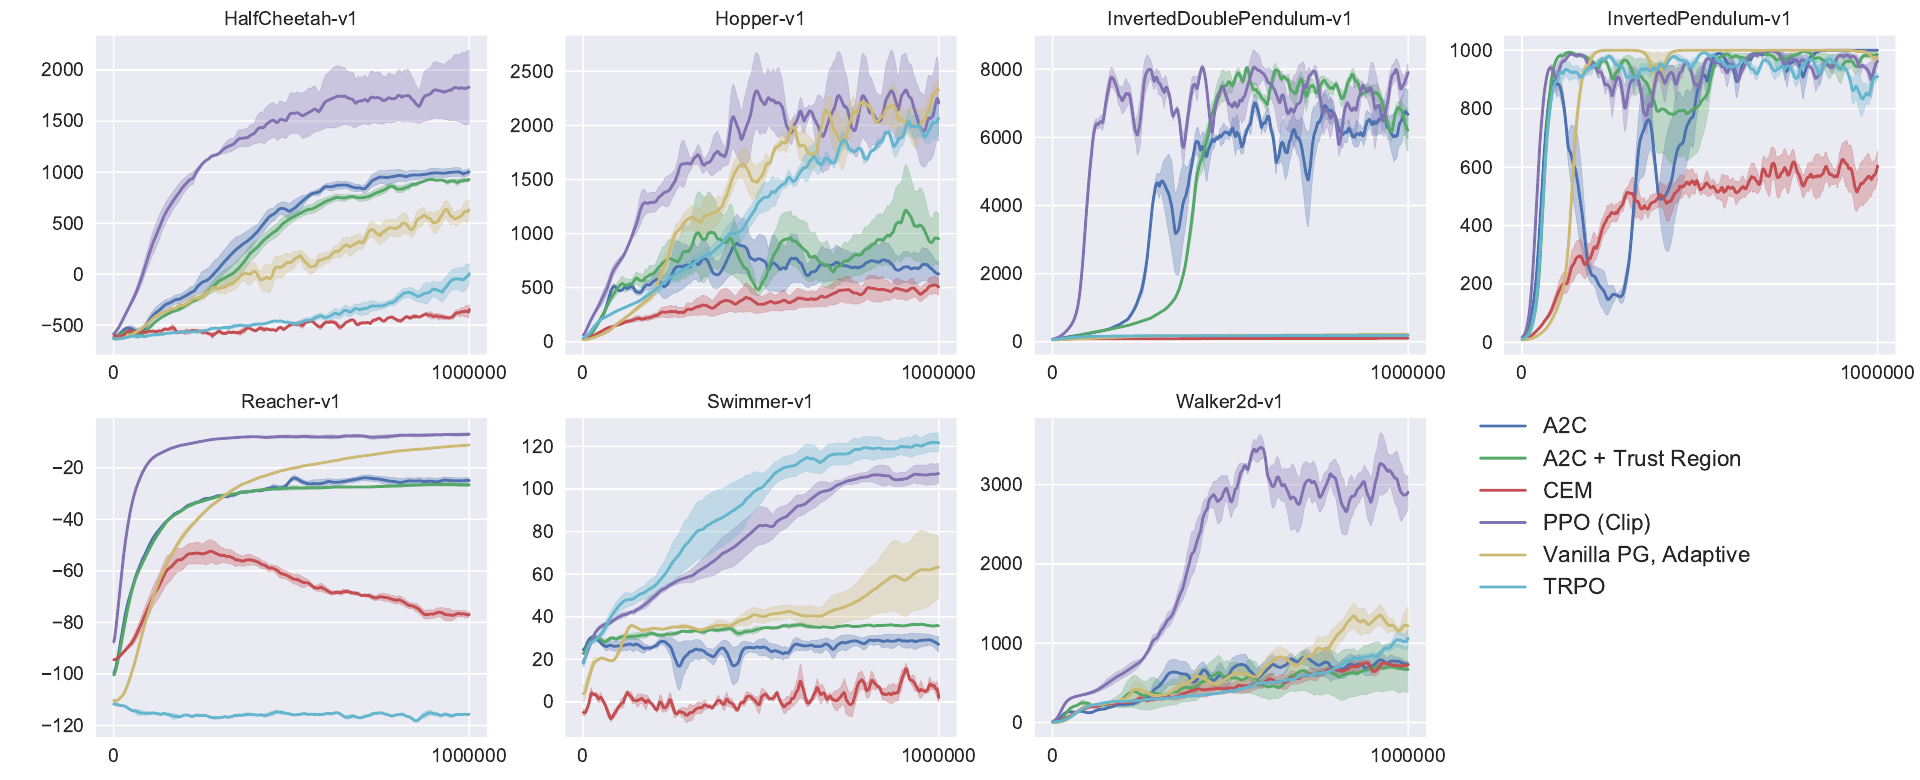
\includegraphics[width=\linewidth]{ppo_fig3_mujoco.png}\\
{\scriptsize PPO Fig.~3: MuJoCo, one million timesteps.}
\end{center}

\begin{minipage}[c]{0.5\linewidth}
\begin{itemize}
  \item \textbf{MuJoCo}: {\color{AtlasCool}\textbf{PPO (clip)}} best on almost all 7 tasks --- above TRPO, A2C, CEM, vanilla PG. Swimmer is the one task where TRPO is clearly ahead.
  \item Also (not shown): 3D humanoid running, steering and getting up.
\end{itemize}
\end{minipage}\hfill
\begin{minipage}[c]{0.46\linewidth}
\centering\small
\textbf{Atari}, 49 games --- games won\\[2pt]
\begin{tabular}{l r r r}
\toprule
 & A2C & ACER & \textbf{PPO} \\
\midrule
avg.\ over training & 1 & 18 & \textbf{30} \\
last 100 episodes & 1 & \textbf{28} & 19 \\
\bottomrule
\end{tabular}\\[2pt]
{\scriptsize ``avg.\ over training'' favors fast learning.}
\end{minipage}

% ---------------------------------------------------------------------------
\section{The whole story: CPI $\to$ TRPO $\to$ GAE $\to$ PPO}
% ---------------------------------------------------------------------------

\begin{center}
\footnotesize
\begin{tabularx}{\linewidth}{@{}>{\bfseries\raggedright\arraybackslash}p{2.6cm} L L L L@{}}
\toprule
 & \textbf{CPI} & \textbf{TRPO} & \textbf{GAE} & \textbf{PPO} \\
\midrule
{\color{AtlasWarm}A.\ how far may I step?} & mixture step $\alpha$ & KL trust region $\delta$ & trust region for $\pi$ \textbf{and} $V$ & clipped ratio $\epsilon$ \\
how is it solved? & greedy chooser + formula for $\alpha$ & CG + line search & CG (policy and value) & Adam, $K$ epochs \\
advantage estimate & rollouts from restarts & Monte Carlo $\hat Q$ & GAE$(\gamma,\lambda)$ + critic & truncated GAE \\
{\color{AtlasCool}B.\ where do states come from?} & {\color{AtlasCool}restarts $s_0\sim\mu$} & {\color{BadRed}$\rho_0$ (vine: resets to visited states)} & {\color{BadRed}$\rho_0$} & {\color{BadRed}$\rho_0$ (+ entropy bonus on actions)} \\
\bottomrule
\end{tabularx}
\end{center}

\begin{enumerate}
  \item \textbf{Row A}: the same idea at every stage --- keep the new policy close to the one that produced the data, because the surrogate uses the old state distribution. By construction (CPI), by a constraint (TRPO), by the objective (PPO).
  \item \textbf{Rows 2--3}: the price of keeping close falls, from a theoretical step size to an off-the-shelf optimizer, and from restart rollouts to a learned critic.
  \item \textbf{Row B}: CPI's second fix is \textbf{not} carried forward.
\end{enumerate}

\subsection{One line per paper}

\begin{center}
\small
\begin{tabularx}{\linewidth}{@{}l L L@{}}
\toprule
\textbf{Paper} & \textbf{Problem it attacks} & \textbf{Main idea} \\
\midrule
\textbf{CPI} & greedy updates from approximate values can hurt & conservative mixture, step $\alpha$ from a bound \\
\textbf{CPI} & on-policy samples miss important states & exploratory restart distribution $\mu$ \\
\textbf{TRPO} & mixtures don't fit neural-net policies & step size $=$ a policy distance (KL) \\
\textbf{TRPO} (practice) & the theoretical penalty is far too conservative & mean-KL trust region, CG + line search \\
{\color{AtlasWarm}\textbf{GAE}} & $\hat A_t$ from returns is too noisy & critic $V$ + bias--variance knob $\lambda$ \\
{\color{AtlasCool}\textbf{PPO}} & second-order step, one step per batch & clipped ratio + minibatch SGD, $K$ epochs \\
\bottomrule
\end{tabularx}
\end{center}

\begin{keybox}[title={Take-home}]
One idea --- \textbf{stay close to the data-generating policy, measured on its own states} --- runs from CPI to PPO, made cheaper at each step. CPI's state-coverage idea was dropped along the way.
\end{keybox}
